\documentclass[a4paper,12pt]{article}
\pagestyle{plain}
\usepackage[T1]{fontenc}
\usepackage{txfonts}
\sloppy
\usepackage{graphicx}
\newcommand{\tab}{\verb+    +}
\begin{document}

\title{Assignment - Module 3}
\date{\today}
\author{Chidambaram P G, Fathima M, Mohan S Nayaka, Muhassin Babu M M\\ Pathang V S, Selvam G, Suraj K}
\maketitle
\noindent
6. Describe and differentiate between synthesised and inherited attributes.\\
\emph{Answer}:

\textbf{Synthesized attributes} are those attributes whose values are only in productions in which their symbol appears on the left-hand side.For annotated parse trees this means that the attribute flow --- the pattern in
which information moves from node to node is entirely bottom-up.    An attribute grammar in which all attributes are synthesized is said to be S-attributed. The arguments to semantic functions in an S-attributed grammar are always attributes of symbols on the right-hand side of the current production, and the return value is always placed into an attribute of the left-hand
side of the production.

Attributes whose values are calculated when their symbol is on the right-hand side of the current production are said to be \textbf{inherited attributes}. They allow contextual information to flow into a symbol from above or from the side, so that the rules of that production can be enforced in different ways (or generate different values) depending on surrounding context. Symbol table information is commonly passed from symbol to symbol by means of inherited attributes. Inherited attributes of the root of the parse tree can also be used to represent the external environment.\\
\\
\\
\\
\noindent
7. Show the stack with all activation record instances, including the dynamic chain, when
execution reaches position 1 in the following skeletal program. This program uses the deep-
access method to implement dynamic scoping.\\
void fun1() \{\\
float a;\\
...\\
\}\\
void fun2() \{\\
int b, c;\\
...\\
\}\\
void fun3() \{\\
float d;\\
... \verb+       + $\longleftarrow$ 1\\
\}\\
void main() \{\\
char e, f, g;\\
...\\
\}\\
The calling sequence for this program for execution to reach fun3 is:\\
main calls fun2\\
fun2 calls fun1\\
fun1 calls fun1\\
fun1 calls fun3\\
\emph{Answer}:\\
If local variables are stack dynamic and are part of the activation records in a
dynamic-scoped language, references to nonlocal variables can be resolved by
searching through the activation record instances of the other subprograms
that are currently active, beginning with the one most recently activated.

The dynamic chain links together all subprogram activation record instances in the reverse of the order in which they were activated. Therefore, the dynamic chain is exactly what is needed to reference
nonlocal variables in a dynamic-scoped language. This method is called deep
access, because access may require searches deep into the stack.

The activation records for the given code example is:\\
\begin{figure}
\centering
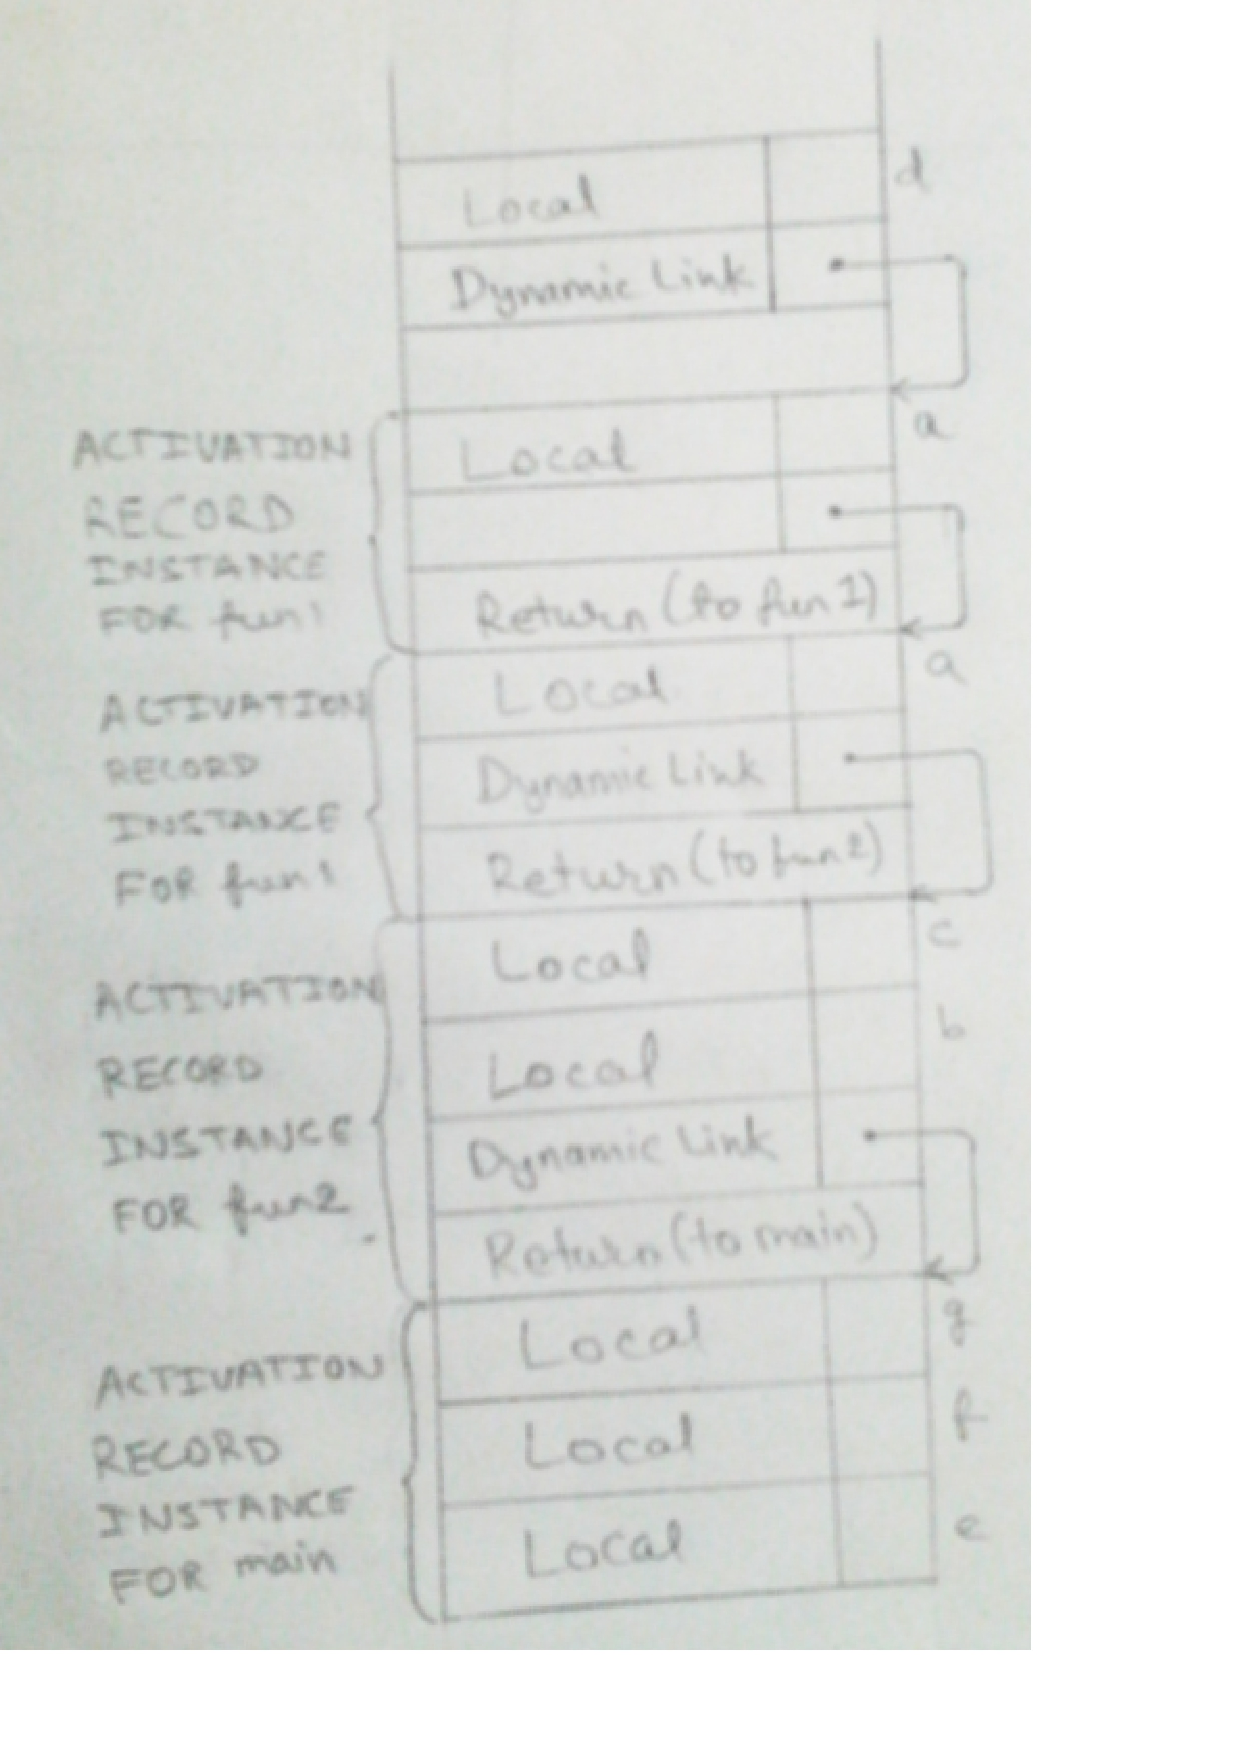
\includegraphics[scale=0.6]{q7}
\end{figure}
\pagebreak
\\
\\
\\
\\
\\
\\
\\
\noindent
8. Design a skeletal program and a calling sequence that results in an activation
   record instance in which the static and dynamic links point to different
   activation-recorded instances in the run-time stack. \\
\emph{Answer}:\\
procedure Main\_2 is\\
\verb+    + X : Integer;\\
\verb+    +procedure Bigsub is\\
\verb+    +\verb+    +    A, B, C : Integer;\\
\verb+    +\verb+    +    procedure Sub1 is\\
\verb+    +\verb+    +\verb+    +    A, D : Integer;\\
\verb+    +\verb+    +\verb+    +    begin -- of Sub1\\
\verb+    +\verb+    +\verb+    +    A := B + C; $\longleftarrow$ 1\\
\verb+    +\verb+    +\verb+    +      ...\\
\verb+    +    end; -- of Sub1\\
\verb+    +    procedure Sub2(X : Integer) is\\
\verb+    +\verb+    +      B, E : Integer;\\
\verb+    +\verb+    +      procedure Sub3 is\\
\verb+    +\verb+    +\verb+    +        C, E : Integer;\\
\verb+    +\verb+    +\verb+    +        begin -- of Sub3\\
\verb+    +\verb+    +\verb+    +        ...\\
\verb+    +\verb+    +\verb+    +        Sub1;\\
\verb+    +\verb+    +\verb+    +        ...\\
\verb+    +\verb+    +\verb+    +        E := B + A; $\longleftarrow$ 2\\
\verb+    +\verb+    +      end; -- of Sub3\\
\verb+    +\verb+    +      begin -- of Sub2\\
\verb+    +\verb+    +      ...\\
\verb+    +\verb+    +      Sub3;\\
\verb+    +\verb+    +      ...\\
\verb+    +\verb+    +      A := D + E; $\longleftarrow$ 3\\
\verb+    +    end; -- of Sub2\\
\verb+    +    begin -- of Bigsub\\
\verb+    +\verb+    +    ...\\
\verb+    +\verb+    +    Sub2(7);\\
\verb+    +\verb+    +    ...\\
\verb+    +  end; -- of Bigsub\\
  begin -- of Main\_2\\
\verb+    +  ...\\
\verb+    +  Bigsub;\\
\verb+    +  ...\\
end; -- of Main\_2\\
\\
The sequence of procedure calls is:\\
Main\_2 calls Bigsub\\
Bigsub calls Sub2\\
Sub2 calls Sub3\\
Sub3 calls Sub1\\
\\
The activation records with static and dynamic links is as follows:\\
\begin{figure}
\centering
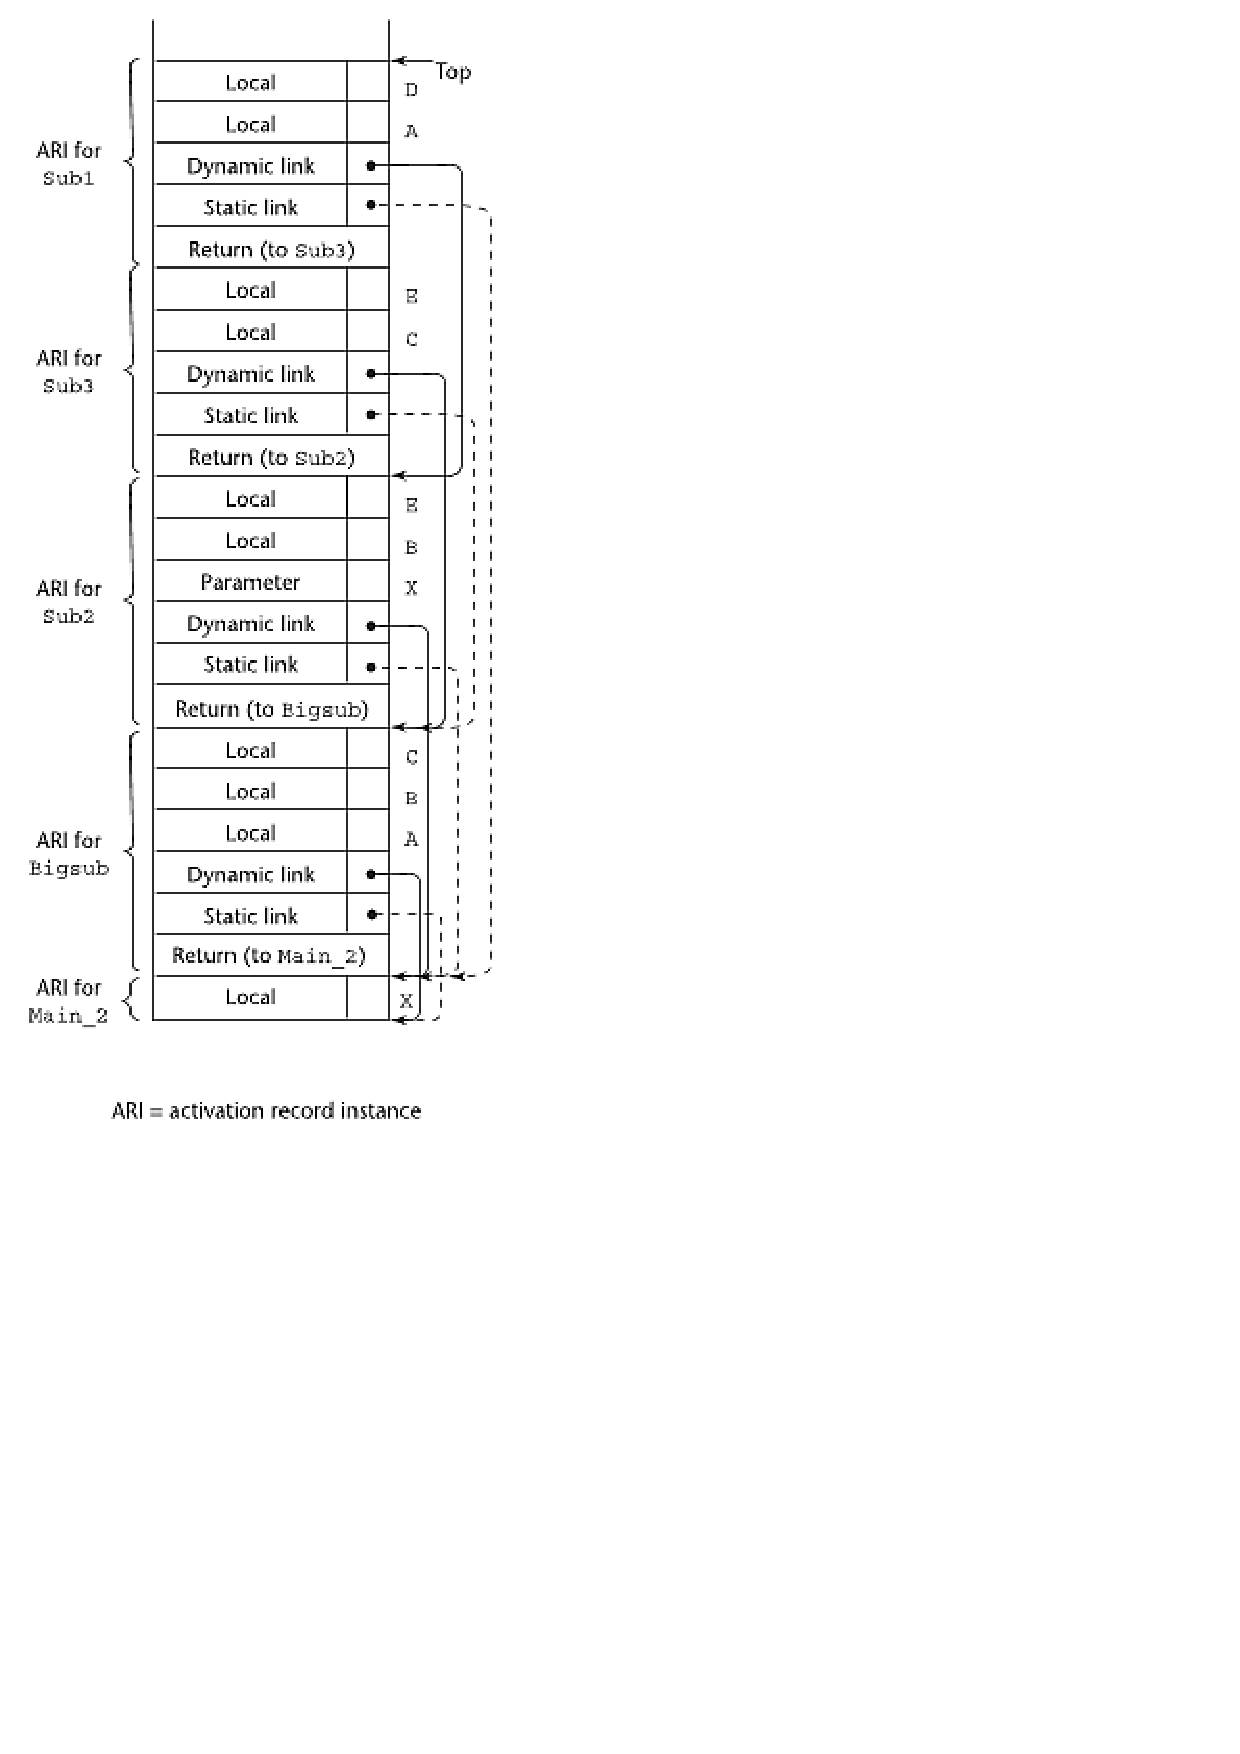
\includegraphics[scale=0.5]{ari}
\end{figure}

     At position 1 in procedure Sub1, the reference is to the local variable,
A, not to the nonlocal variable A from Bigsub. This reference to A has the
chain\_offset/local\_offset pair (0, 3). The reference to B is to the nonlocal B
from Bigsub. It can be represented by the pair (1, 4). The local\_offset is 4,
because a 3 offset would be the first local variable (Bigsub has no parameters). Notice that if the dynamic link were used to do a simple search for
an activation record instance with a declaration for the variable B, it would
find the variable B declared in Sub2, which would be incorrect. If the (1, 4)
pair were used with the dynamic chain, the variable E from Sub3 would be
used. The static link, however, points to the activation record for Bigsub,
which has the correct version of B . The variable B in Sub2 is not in the
referencing environment at this point and is (correctly) not accessible. The
reference to C at point 1 is to the C defined in Bigsub, which is represented
by the pair (1, 5).\\
\\
\noindent
9. What does it mean for an attribute grammar to be S-attributed? L-attributed? Noncircular? What is the significance of these grammar classes?
\\
\emph{Answer}:\\
   An attribute grammar in which all attributes are synthesized is said to be \textbf{S-attributed}. The arguments to semantic functions in an S-attributed grammar are always attributes of symbols on the right-hand side of the current production, and the return value is always placed into an attribute of the left-hand side of the production. Tokens (terminals) often have intrinsic properties (e.g.,
the character-string representation of an identifier or the value of a numeric constant); in a compiler these are synthesized attributes initialized by the scanner.

An \textbf{L-attributed} grammar is where attributes can be evaluated by visiting the nodes of the parse tree in a single left-to-right, depth-first traversal (the same order in which they are visited during a top-down parse). \\Formally, it follows the following rules:\\
\begin{itemize}
\item Each synthesized attribute of of a left-hand side symbol depends only on that symbol's inherited attributes or on attributes (synthesized or inherited) of the the production's right-hand side symbols; and
\item each inherited attribute of a right-hand side symbol depends only on inherited attributes of the left-hand side symbol or on attributes (synthesized or inherited) of symbols to its left on the right-hand side.
\end{itemize}

An attribute grammar is \textit{noncircular} if it never leads to a parse tree in which there are cycles in the attribute
flow graph --- that is, if no attribute, in any parse tree, ever depends (transitively) on itself.

\textbf{Significance}:    S-attributed grammars are the most general class of attribute grammars for which evaluation can be implemented on-the-fly during an LR parse. L-attributed grammars are a proper superset of S-attributed grammars. They are the most general class of attribute grammars for which evaluation can be implemented on-the-fly during an LL parse.\\
\\
\noindent
10. Explain Space Management Atrributes for Context-free grammar for a calculator language.\\
\emph{Answer}:\\
Any attribute evaluation method requires space to hold the attributes of the
grammar symbols. If we are building an explicit parse tree, then the obvious approach is to store attributes in the nodes of the tree themselves. If we are not building a parse tree, then we need to find a way to keep track of the attributes
for the symbols we have seen (or predicted) but not yet finished parsing. The details differ in bottom-up and top-down parsers.

For a bottom-up parser with an S-attributed grammar:
\begin{itemize}
\item maintain an attribute stack that directly mirrors the parse stack
\begin{itemize}
\item next to every state number on the parse stack is an attribute record for the symbol we shifted when we entered that state.
\end {itemize}
\end {itemize}

The context-free grammar for a calculator language is:\\
\begin{quote}
1. $E_1$ $\longrightarrow$ $E_2$ + T \\
\verb+       +$\triangleright$ $E_1$.val := sum($E_2$.val + T.val)\\
2. $E_1$ $\longrightarrow$ $E_2$ - T \\
\verb+       +$\triangleright$ $E_1$.val := sum($E_2$.val - T.val)\\
3. E $\longrightarrow$  T \\
\verb+       +$\triangleright$ E.val := T.val\\
4. $T_1$ $\longrightarrow$ $T_2$ * F \\
\verb+       +$\triangleright$ $T_1$.val := product($T_2$.val * F.val)\\
5. $T_1$ $\longrightarrow$ $T_2$ / F \\
\verb+       +$\triangleright$ $T_1$.val := quotient($T_2$.val / F.val)\\
6. T $\longrightarrow$  F \\
\verb+       +$\triangleright$ T.val := F.val\\
7. $F_1$ $\longrightarrow$ $-F_2$\\
\verb+       +$\triangleright$ $F_1$.val := additive\_inverse($F_2$.val)\\
8. F $\longrightarrow$  (E) \\
\verb+       +$\triangleright$ F.val := E.val\\
9. F $\longrightarrow$ const
\verb+       +$\triangleright$ F.val := const\\
\end{quote}
We can use the approach described above for bottom-up parser and all the attributes in this grammar are synthesized.
For example, consider the parse tree below for the expression (1+3) * 2. The val attributes of symbols are shown in boxes. Curved arrows represent the attribute flow, which is strictly upward in this case.
\begin{figure}[!hbp]
\centering
\includegraphics[scale=0.45]{agq10}
\caption{Decoration of a parse tree for (1 + 3) * 2 }
\end{figure}
\end{document}
